At the basic level our project has not only met, but far surpassed the criteria we set for it to achieve. However, we need to take a broader based approach at our evaluation of our projects success by comparing it with similar commercial products which are currently on the market. 

Our target was for the project to have all features from the realistic best version (v2) and a few from the ideal version (v3), which it easily met.  With a sizable database composed of over 900 recipes, our product rivals many commercial products of similar scope.

Moreover, our product offers auto-complete based search of ingredients, which gives users an early affirmation when they attempt to search for a recipe based on their ingredients. This is unlike most similar products on the market, like BBC recipes and RecipeZaar.com. Supercook.com does offer auto-complete of ingredients, however, our website does it a step better because we allow the ingredient to form a `token', which is visually more appealing than the one used on Supercook.com. (refer to diagram).

\begin{figure}[h]
\begin{center}
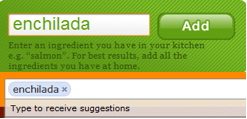
\includegraphics[width=0.5\textwidth]{autocomplete}
\caption{The auto complete search field for Supercook.com }
\end{center}
\end{figure}

Additionally, our project avoids clutter, with which most websites of similar scope are plagued, for example recipeZaar.com. With a user's short attention span, purging superfluous information from our website prevents distracting users when they use our services.

Our index page features a slideshow which, upon refreshing the page, generates a completely new list of featured recipes, which you can quickly browse through pictorially, which encourages more ambitious users to create recipes which they would normally have never chanced upon. Serendipity is an important part of our website.  As another example, by setting up an account with us, users are recommended recipes based on collaborative filtering technology, which provides users with seemingly `coincidental' recipes which they are likely to enjoy. This feature rivals many commercial websites, some of which, like BBC Recipes, do not even provide this functionality.

We have also used taken human behaviour into account when designing the website, decorating our interface with appetite stimulating colours like orange. Moreover, our banner spells `Digichef' using fruits and vegetables, alongside our mascot, which is a chef-robot. The central idea behind this was that if we are successful in stimulating the user's appetite while at the same time, marketing our mascot , we will be able to build a customer base who are more likely to repeatedly visit our website. No other website features a mascot, which in our opinion, presents an untapped resource to use for marketing purposes. 

 In addition, we allow users to set up an account with us, where users can upload their own recipes. There might be a potential problem here if users are allowed to submit any recipe of substandard quality. To solve this, we implemented a voting feature, where users can express their opinion on a recipe. Allowed more time, our group could have implemented more social networking features like chat to provide an involved user experience.

The search returns a list of recipes; each recipe contains a list of ingredients, instructions, and the ability to vote the recipe and also includes recipes similar to the recipe selected. Every recipe includes an image; for testing purposes we collected images from Google Image Search using a custom script and stored these as URLs within the database. Although this works well for the current version, if we had more time and a larger design team we would have been able to create a database of images for the recipes. 

The banner uses different ingredients to spell DigiChef; this design emphasizes the purpose of the website. The colour scheme used is white, yellow and orange. The white background emphasises simplicity and clarity, this is an important criterion for retaining the attention of the user.  Moreover, research suggests that the orange colour is stimulating for the users appetite.\footnote{[Link to research, 31st March 2010 \url{http://desktoppub.about.com/cs/colorselection/p/orange.htm}]} 


We have also implemented user accounts using a module called auth that handles users and their accounts. Users create a user account specifying their username, password, an about them section, their gender, email account, and their first and last name. This function has been implemented using a module called registration. The profile page includes the about them section, recipes that the user has liked and recommendations. Having a user account allows the user to rate recipes that they like or hate, these ratings are taken into consideration when the user searches for a recipe and returns only recipes that the user is most likely going to like. These functionalities introduce the use of Collaborative Filtering, this being something that not all of the recipe websites mentioned in our research include. 
